\section{Planning the review}
\label{section:Planning}

To collect all the information needed for a better understanding of the main problem and approaches that have been used, a \acrfull{SLR} was conducted through a transparent process, avoiding biases and increasing reliability.

The three steps process used in the literature review were: a (i) planning stage, where the need for a review was addressed, the researches questions were summarized into search terms, and a specific review protocol was created beforehand; therefore the (ii) review was conducted, identifying the researches which aimed to solve the slot allocation problem, selecting the primary studies, verifying their quality assessments, extracting the data, and synthesizing its information; after the (iii) review result was presented, in order to state what are the main researches in the central problem, and how the methods here presented can fulfill some of the gaps left in the previous literature.

A better understanding of the airports' slot allocation problem, through a literature review, is needed in order to identify, analyze and interpret the different perspectives of the problem and how it has been approached, aiming to set the historical context and present how this paper can contribute for the problem solution. To achieve this objective, through a process that mitigate bias, conducting the data gathering in a transparent way, the review criteria and its steps were planned before their execution, following the guidelines presented in \cite{wohlin2012experimentation}. The \refFig{fig:experiment} presents the processes followed and their deliverables.

\figuraBib{10_literaturaReview_en}{The literature review processes and their deliverables}{wohlin2012experimentation}{fig:experiment}{width=0.6\textwidth}%

\subsection{The need for a review}

The first step was the identification of the need for a review, i.e., understand how the problem has been addressed in past research and what are the previous limitation. It is common for airports to have different infrastructure configurations, i.e., runways, taxiways, gates, terminals. Also, different airports are placed in different environments, such as populated areas, which plays a critical role in their demand. Such specificities can introduce different points of view for the slot allocation, and it is expected different proposed solutions. Since the current paper raises a well-established problem, it is necessary to understand how it has been historically managed. Although a literature review could be achieved directly through a \textit{snowballing} process, it would only collect some points of view, introducing a search bias that could affect its reproducibility. A systematic review provides a better approach, resulting in a comprehensive understanding of the problem, delivered by a step-by-step protocol, which can be reviewed and improved. In this step of the review, it is assumed that no systematic review was made before, but if encountered it would be evaluated its contributions and limitations

\subsection{The \acrshort{SLR} researches questions}

The second step was the specification of research questions for the search conducted in the literature review. These questions set focus for the identification of the primary studies, as well as the extraction and analysis of the studies' information. To guarantee focus, PICO was used to break the questions down to their essential parts. It was also set an experimental design in the intervention part, in order to clarify what was the present paper approach, in the case it has been already used. In this step were produced the following research questions for the literature review:
\begin{itemize}
    \item \textbf{RQ1:} For the airports' slot allocation problem (P), what are the current approaches (I) that can provide an optimization in the initial slot allocation process (O)?
    \item \textbf{RQ2:} For the airports' slot allocation problem (P), can a methodology using integer programming or machine learning (I) provide the better optimal solution, reducing negative impacts for airlines' initial allocation (O), than the current approaches (C)?
\end{itemize}

The question one can be divided in three specific question: (i) what the methodology used to solve the airport slot allocation problem? (ii) what are the constraints to the approaches? (iii) Are there any gaps or assumptions that could be explored?
The second question wants to collect all information about models of the problem and how experimentation with algorithms are helping to tackle them.

\subsection{Review protocol}

The third, and last step for the planning part, was the development of a review protocol. This section acts not only as a backbone for the present paper research review but also is important for its reproducibility and validity evaluation. The following items, beyond the background and research question for the review addressed above, were taken into consideration:

\subsubsection{Search strategy for primary studies}

The main activities in this step are specifying the search string through the research question for the literature review, and applying this string in databases. The string used is a composition of the keywords: Airport, Slot, allocation, integer programming, machine learning, optimization, and solution. Treating the bag of words with search operators, the following search string was created: 
\\

\textit{(airport* \textbf{AND} "slot allocation" \textbf{AND}
 optimization \textbf{AND} ("machine learning" \textbf{OR} "integer programming"))}. 
\\

\subsubsection{Search sources}

This string should be used in the following databases in order to collect the primary researches:
\begin{enumerate}
    \item ACM Digital Library;
    \item \acrfull{BASE};
    \item EBSCO;
    \item ScienceDirect;
    \item Scopus;
    \item \acrfull{TRID};
    \item Web of Science;
    \item CiteSeerX;
    \item \acrfull{DBLP};
    \item \acrfull{DOAJ};
    \item IEEE Xplore;
    \item JSTOR; and
    \item Springer Link (Article section).
\end{enumerate}


There are two main criteria for selecting these databases: (i) they cover multidisciplinary subjects, or their specialized field are related with computer science or transportation studies, which are the main areas of the present paper; and (ii) these databases were described in \cite{kitchenham2007guidelines} by their coverage and capability to perform systematic searches via queries and filter, so that the final result of using this databases is a reproducible, with high recall and precision.  

The \cite{gusenbauer2020academic} presents the databases as primary if they fulfill all the necessary quality requirements, such as the possibility of query refinement, string size criteria, server response criteria, use of Boolean operators, functionalities and reproducibility, otherwise they are considered supplementary. The databases 1 to 7 are primary databases and the other ones are supplementary. Additional search can be conducted in specific journals and conferences, as well as contacting researchers for aggregating material yet not published and grey literature. All additional material must be specified with its origin, in the interest of maintaining the reproducibility of the review.

In this step, all identifiable false positives and duplicates between databases have to be removed. To validate the search string, the article \cite{ribeiro2018optimization}, which was already evaluated as a positive result, must be contained in one of the results of the databases, otherwise, a string reformulation is needed.

\subsubsection{Study selection criteria}

Some selection criteria of inclusion and exclusion were established beforehand to mitigate bias. Using the "First pass" approach \cite{keshav2007read} all the primary papers' titles, abstracts,introductions and conclusions will be read. 
Articles are going to be included if they contain: 
\begin{enumerate}
    \item Any aspect of airport's slot allocation problem (models, perspectives, constraints, methods, technical consideration, etc.); and
    \item Any solution for the airports' slot allocation problem using integer programming or machine learning.
\end{enumerate}

\subsubsection{Study exclusion criteria}

Articles are going to be excluded if: 
\begin{enumerate}
    \item They are duplicates or old versions (If it is found in more than one primary and/or secondary, it is kept in the databases sorted as shown in the topic 'Search sources' and removed from the others);
    \item They were produced before 2001 (Commercial flights market regulation after the September 11 attack);
    \item They are introducing new slot guidelines besides those explained in the IATA's WASG \cite{WASG2020};
    \item They contain methods that solve Airports' slot problem through auction (Economic approaches); 
    \item They are not accessible in full-text;
    \item They are not related with the research questions, nor are tackling the main problem, but adjacent areas (ground delays, weather impacts in airports, etc.);
    \item They have a specific context (September 11 attacks, COVID-19 pandemic, etc.); and
    \item They are not in English nor Portuguese.
\end{enumerate}

\subsubsection{Study selection procedures}

The first step of the selection is remove all papers that are obviously not relevant. After, it will be conducted by the main research assessment of each paper, using the selection and exclusion criteria, with a random samples of the paper. If more than one section of the paper fail to be relevant for the present review, the paper will be removed and a justification will be written.


\subsubsection{Study quality assessment checklist and procedures}

In addition to the selection procedures, it was established the assessment of the quality of the primary studies. The quality provides a better understand of the differences between studies, given importance to those which follow high level criteria. Kitchenham and Charters (\citeyear{kitchenham2007guidelines}) present a quality questionnaire based on 5 issues affecting the quality of the study, given 5 for a 'Yes' and 0 for a 'No' answer:
    \begin{itemize}
    \item \textbf{QQ1:} Is the data analysis process appropriate?
    \item \textbf{QQ2:} Did studies carry out a sensitivity or residual analysis?
    \item \textbf{QQ3:} Were accuracy statistics based on the raw data scale?
    \item \textbf{QQ4:} Was the data selected at random (not selected for convenience) from several airports?
    \item \textbf{QQ5:} How many datasets were used? Evaluation: More than 10 = 5; More than 1 but less than 10 = 1; and only one dataset = 0.
    \end{itemize}

It was also cited the reporting quality based on 4 questions \cite{kitchenham2007guidelines}, which were giving less weight, (1) for a 'Yes' and (-1) for a 'No' answer, than those that measure the study quality:
    \begin{itemize}
    \item \textbf{RQ1:} Is it clear what projects were used to construct each model?
    \item \textbf{RQ2:} Is it clear how accuracy was measured?
    \item \textbf{RQ3:} Is it clear what cross-validation method was used?
    \item \textbf{RQ4:} Were all model construction methods fully defined (tools and methods used)?
    \end{itemize}

\subsubsection{Data extraction strategy}

Data extraction was defined as a set of information that should be extracted for each study. This data are important for any attempt to summarize the results. 

The following data, and their specific contexts, will be extract:

\begin{enumerate}
    \item (Design) Method used
    \item(Conduct) Description of the data collection methods
    \item(Conduct) If two "groups" are being compared, were they treat similarly in the study?
    \item(Analysis) Was the statistical significance assessed?
    \item(Conclusion) Are all the answered question answered?
    \item(Conclusion) Are negative findings presented?
    \item(Conclusion) How do results add to the literature?
\end{enumerate}


\section{Conducting the review}
\label{section:Conducting}
This section reports the outcome of the systematic search and selection process. It also presents the validity checks, including the data extraction and quality assessment process.

\subsection{Identification of research}

The research found 176 sources in 13 databases. It was found 30 duplicates (17.04\%), which were excluded from the review, resulting in 146 unique sources, as shown in the Table \ref{table*:results}.

\begin{table*}[h]
\begin{center}
\caption{Search results per database}
\small
\begin{tabular}{*{15}{l}}
\hline
\multicolumn{1}{l}{\#} & \textbf{DATABASE}                                     & \multicolumn{1}{l}{\textbf{SOURCES FOUND}} \\ \hline
1  & ACM Digital Library                      & 20 \\
2  & Bielefeld Academic Search Engine (BASE)  & 8  \\
3  & EBSCO                                    & 20 \\
4  & ScienceDirect                            & 74 \\
5  & Scopus                                   & 8  \\
6                      & Transport Research International Documentation (TRID) & 8                                          \\
7  & Web of Science                           & 6  \\
8  & CiteSeerX                                & 0  \\
9                      & Digital Bibliography \& Library Project (DBLP)        & 8                                          \\
10 & Directory of Open Access Journals (DOAJ) & 3  \\
11 & IEEE Xplore                              & 1  \\
12 & JSTOR                                    & 1  \\
13 & Springer Link                                         & 19                     \\ \hline
   & \textbf{TOTAL}                                        & 146                    \\ \hline
\end{tabular}
\label{table*:results}
\end{center}
\end{table*} 

Most of the studies were found in the primary databases 81,81\%, being the main source the ScienceDirect with 42,04\% of total. The more specialized sources performed worst, collecting less studies related with slot allocation in airports, such as \acrshort{TRID} (transportation) and IEEE Xplore (computing science), which found 4.54\% and 0.56\% of the total, respectively. 

Therefore, scrutiny was necessary to streamline these studies to relevant ones. Using the "first pass" \cite{wohlin2012experimentation}, the title of each study and their contents were briefly analyzed separately and randomly. Hence, all the papers that do not reflect the discussion about airport slot allocation problem or were unable to pass through the exclusion criteria were removed. The result was the identification of 47 primary studies, which is 26.70\% of the total first found.
\\

For the exclusion criteria: 
\begin{enumerate}
    \item One editorial was removed due to its scope being very wide, not detailing methods (1.01\%);
    \item One article was not accessible (1.01\%);
    \item Two articles were removed due to the year of publication (2.02\%);
    \item 18 studies were not related with the airports' slot allocation problems (18.18\%);
    \item 30 studies were solving the slot allocation problem with economic approaches (30.30\%), such as auctions (25 out of 30); and
    \item 46 studies were focusing in adjacent area (47.47\%), such as ground delays (10 out of 47).
\end{enumerate}

After the selection procedure, the SLR resulted in 47 primary studies, showing a high number of primary false positives studies, i.e., studies that were brought by the research string but should not have been. The table \ref{table*:falsepositive} shows the primary studies per database and the false positive result, after the removal of the duplicates. After the duplication removal and exclusion criteria, Scopus, Web of Science, IEEE Xplore, and JSTOR ran out of studies. The overall primary false positive result was of 67.81\%, indicating that the search was comprehensive. 


\begin{center}
    
\setlength{\tabcolsep}{10pt} % Default value: 6pt
\renewcommand{\arraystretch}{1.5} % Default value: 1
\begin{xltabular}{\textwidth}{p{0.5cm} p{7cm} p{3cm} p{2.6cm}}
\caption{Primary studies per database and the false positive results.} \label{table*:falsepositive} \\

\hline \multicolumn{1}{c}{\#} & \textbf{DATABASE}                                     & \textbf{PRIMARY STUDIES} & \textbf{FALSE POSITIVES} \\ \hline 
\endfirsthead

\multicolumn{4}{c}%
{\tablename\ \thetable{} - Continued from previous page.} \\
\hline \multicolumn{1}{c}{\#} & \textbf{DATABASE}                                     & \textbf{PRIMARY STUDIES} & \textbf{FALSE POSITIVES} \\ \hline 
\endhead

\hline \multicolumn{4}{r}{{Continued on next page.}} \\ \hline
\endfoot

\hline
\endlastfoot

1                    & ACM Digital Library                            & 4  & 80.00\%     \\
2                    & Bielefeld Academic Search Engine (BASE)        & 4  & 50.00\%  \\
3                    & EBSCO                                          & 3  & 83.33\%  \\
4                    & ScienceDirect                                  & 30 & 58.33\%  \\
5                    & Scopus                                         & 0  & -   \\
6                      & Transport Research International Documentation (TRID) & 2                                            & 0.00\%                   \\
7                    & Web of Science                                 & 0  & -        \\
8                    & CiteSeerX                                      & 0  & -        \\
9                    & Digital Bibliography \& Library Project (DBLP) & 1  & 66.67\%  \\
10                   & Directory of Open Access Journals (DOAJ)       & 1  & 33.33\%  \\
11                   & IEEE Xplore                                    & 0  & -        \\
12                   & JSTOR                                          & 0  & - \\
13                   & Springer Link                                  & 2  & 88.89\%  \\ \hline
\multicolumn{1}{l}{} & \textbf{TOTAL}                                          & 47 & 67.81\%  \\ \hline
\end{xltabular}

\end{center}

The number of studies by year of publication is depicted in \refFig{fig:yearPublication}. The topic "airports' slot allocation" have been highlighted in recent years with 74,47\% of the studies selected being published in the last 5 years (2016-2021). The studied selection procedures are illustrated in the \refFig{fig:resumeSLR}.

\figuraBib{12_yearPublication}{Number of papers by year of publication}{}{fig:yearPublication}{width=0.8\textwidth}%

\begin{wrapfigure}{L}{6cm}
\caption{The studies selection procedures and deliverable.}\label{fig:resumeSLR}
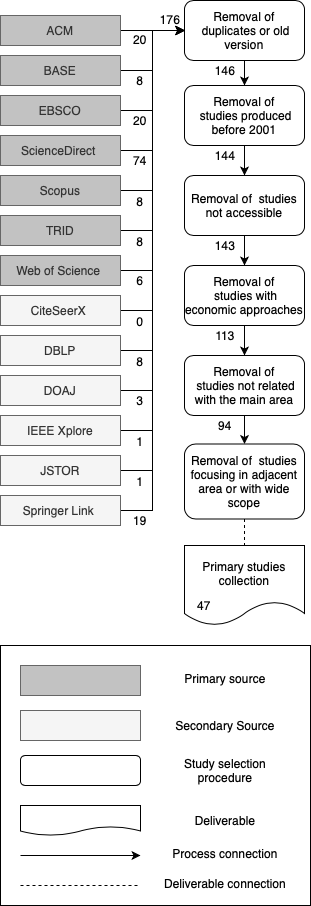
\includegraphics[width=5.25cm]{11_SLR_brief}
\end{wrapfigure} 

\lipsum[1-2]

